\documentclass[]{article}
\usepackage{lmodern}
\usepackage{amssymb,amsmath}
\usepackage{ifxetex,ifluatex}
\usepackage{fixltx2e} % provides \textsubscript
\ifnum 0\ifxetex 1\fi\ifluatex 1\fi=0 % if pdftex
  \usepackage[T1]{fontenc}
  \usepackage[utf8]{inputenc}
\else % if luatex or xelatex
  \ifxetex
    \usepackage{mathspec}
  \else
    \usepackage{fontspec}
  \fi
  \defaultfontfeatures{Ligatures=TeX,Scale=MatchLowercase}
\fi
% use upquote if available, for straight quotes in verbatim environments
\IfFileExists{upquote.sty}{\usepackage{upquote}}{}
% use microtype if available
\IfFileExists{microtype.sty}{%
\usepackage{microtype}
\UseMicrotypeSet[protrusion]{basicmath} % disable protrusion for tt fonts
}{}
\usepackage[margin=1in]{geometry}
\usepackage{hyperref}
\hypersetup{unicode=true,
            pdftitle={Visualizations in R},
            pdfauthor={Mette Langaas and Julia Debik, Department of Mathematical Sciences, NTNU},
            pdfborder={0 0 0},
            breaklinks=true}
\urlstyle{same}  % don't use monospace font for urls
\usepackage{color}
\usepackage{fancyvrb}
\newcommand{\VerbBar}{|}
\newcommand{\VERB}{\Verb[commandchars=\\\{\}]}
\DefineVerbatimEnvironment{Highlighting}{Verbatim}{commandchars=\\\{\}}
% Add ',fontsize=\small' for more characters per line
\usepackage{framed}
\definecolor{shadecolor}{RGB}{248,248,248}
\newenvironment{Shaded}{\begin{snugshade}}{\end{snugshade}}
\newcommand{\KeywordTok}[1]{\textcolor[rgb]{0.13,0.29,0.53}{\textbf{#1}}}
\newcommand{\DataTypeTok}[1]{\textcolor[rgb]{0.13,0.29,0.53}{#1}}
\newcommand{\DecValTok}[1]{\textcolor[rgb]{0.00,0.00,0.81}{#1}}
\newcommand{\BaseNTok}[1]{\textcolor[rgb]{0.00,0.00,0.81}{#1}}
\newcommand{\FloatTok}[1]{\textcolor[rgb]{0.00,0.00,0.81}{#1}}
\newcommand{\ConstantTok}[1]{\textcolor[rgb]{0.00,0.00,0.00}{#1}}
\newcommand{\CharTok}[1]{\textcolor[rgb]{0.31,0.60,0.02}{#1}}
\newcommand{\SpecialCharTok}[1]{\textcolor[rgb]{0.00,0.00,0.00}{#1}}
\newcommand{\StringTok}[1]{\textcolor[rgb]{0.31,0.60,0.02}{#1}}
\newcommand{\VerbatimStringTok}[1]{\textcolor[rgb]{0.31,0.60,0.02}{#1}}
\newcommand{\SpecialStringTok}[1]{\textcolor[rgb]{0.31,0.60,0.02}{#1}}
\newcommand{\ImportTok}[1]{#1}
\newcommand{\CommentTok}[1]{\textcolor[rgb]{0.56,0.35,0.01}{\textit{#1}}}
\newcommand{\DocumentationTok}[1]{\textcolor[rgb]{0.56,0.35,0.01}{\textbf{\textit{#1}}}}
\newcommand{\AnnotationTok}[1]{\textcolor[rgb]{0.56,0.35,0.01}{\textbf{\textit{#1}}}}
\newcommand{\CommentVarTok}[1]{\textcolor[rgb]{0.56,0.35,0.01}{\textbf{\textit{#1}}}}
\newcommand{\OtherTok}[1]{\textcolor[rgb]{0.56,0.35,0.01}{#1}}
\newcommand{\FunctionTok}[1]{\textcolor[rgb]{0.00,0.00,0.00}{#1}}
\newcommand{\VariableTok}[1]{\textcolor[rgb]{0.00,0.00,0.00}{#1}}
\newcommand{\ControlFlowTok}[1]{\textcolor[rgb]{0.13,0.29,0.53}{\textbf{#1}}}
\newcommand{\OperatorTok}[1]{\textcolor[rgb]{0.81,0.36,0.00}{\textbf{#1}}}
\newcommand{\BuiltInTok}[1]{#1}
\newcommand{\ExtensionTok}[1]{#1}
\newcommand{\PreprocessorTok}[1]{\textcolor[rgb]{0.56,0.35,0.01}{\textit{#1}}}
\newcommand{\AttributeTok}[1]{\textcolor[rgb]{0.77,0.63,0.00}{#1}}
\newcommand{\RegionMarkerTok}[1]{#1}
\newcommand{\InformationTok}[1]{\textcolor[rgb]{0.56,0.35,0.01}{\textbf{\textit{#1}}}}
\newcommand{\WarningTok}[1]{\textcolor[rgb]{0.56,0.35,0.01}{\textbf{\textit{#1}}}}
\newcommand{\AlertTok}[1]{\textcolor[rgb]{0.94,0.16,0.16}{#1}}
\newcommand{\ErrorTok}[1]{\textcolor[rgb]{0.64,0.00,0.00}{\textbf{#1}}}
\newcommand{\NormalTok}[1]{#1}
\usepackage{graphicx,grffile}
\makeatletter
\def\maxwidth{\ifdim\Gin@nat@width>\linewidth\linewidth\else\Gin@nat@width\fi}
\def\maxheight{\ifdim\Gin@nat@height>\textheight\textheight\else\Gin@nat@height\fi}
\makeatother
% Scale images if necessary, so that they will not overflow the page
% margins by default, and it is still possible to overwrite the defaults
% using explicit options in \includegraphics[width, height, ...]{}
\setkeys{Gin}{width=\maxwidth,height=\maxheight,keepaspectratio}
\IfFileExists{parskip.sty}{%
\usepackage{parskip}
}{% else
\setlength{\parindent}{0pt}
\setlength{\parskip}{6pt plus 2pt minus 1pt}
}
\setlength{\emergencystretch}{3em}  % prevent overfull lines
\providecommand{\tightlist}{%
  \setlength{\itemsep}{0pt}\setlength{\parskip}{0pt}}
\setcounter{secnumdepth}{0}
% Redefines (sub)paragraphs to behave more like sections
\ifx\paragraph\undefined\else
\let\oldparagraph\paragraph
\renewcommand{\paragraph}[1]{\oldparagraph{#1}\mbox{}}
\fi
\ifx\subparagraph\undefined\else
\let\oldsubparagraph\subparagraph
\renewcommand{\subparagraph}[1]{\oldsubparagraph{#1}\mbox{}}
\fi

%%% Use protect on footnotes to avoid problems with footnotes in titles
\let\rmarkdownfootnote\footnote%
\def\footnote{\protect\rmarkdownfootnote}

%%% Change title format to be more compact
\usepackage{titling}

% Create subtitle command for use in maketitle
\newcommand{\subtitle}[1]{
  \posttitle{
    \begin{center}\large#1\end{center}
    }
}

\setlength{\droptitle}{-2em}

  \title{Visualizations in R}
    \pretitle{\vspace{\droptitle}\centering\huge}
  \posttitle{\par}
  \subtitle{TMA4268 Statistical Learning V2019. Module 1: INTRODUCTION TO
STATISTICAL LEARNING}
  \author{Mette Langaas and Julia Debik, Department of Mathematical Sciences, NTNU}
    \preauthor{\centering\large\emph}
  \postauthor{\par}
      \predate{\centering\large\emph}
  \postdate{\par}
    \date{week 2, 2019}


\begin{document}
\maketitle

{
\setcounter{tocdepth}{2}
\tableofcontents
}
\section{Introduction}\label{introduction}

For each of the plots (scatter plot, histogram, boxplot, area chart,
heat map, correlogram) \emph{explain what you see (including what is on
the x- and y-axis) and try to transform what you see into insight about
the data}. All except the correlogram use \texttt{ggplot2} for plotting.
If you want to read more about the idea behind \texttt{ggplot2} (grammar
of graphics) Chapter 3 of \href{}{R for Data Science} is a good read.

\subsection{Packages needed}\label{packages-needed}

\begin{Shaded}
\begin{Highlighting}[]
\KeywordTok{install.packages}\NormalTok{(}\StringTok{"car"}\NormalTok{)}
\KeywordTok{install.packages}\NormalTok{(}\StringTok{"faraway"}\NormalTok{)}
\KeywordTok{install.packages}\NormalTok{(}\StringTok{"ggplot2"}\NormalTok{)}
\KeywordTok{install.packages}\NormalTok{(}\StringTok{"GGally"}\NormalTok{)}
\KeywordTok{install.packages}\NormalTok{(}\StringTok{"reshape"}\NormalTok{)}
\KeywordTok{install.packages}\NormalTok{(}\StringTok{"corrplot"}\NormalTok{)}
\KeywordTok{install.packages}\NormalTok{(}\StringTok{"corrgram"}\NormalTok{)}
\end{Highlighting}
\end{Shaded}

\subsection{Data sets}\label{data-sets}

Three different data sets are used - read descriptions in R:

\begin{itemize}
\tightlist
\item
  \texttt{SLID}: \texttt{?car::SLID}
\item
  \texttt{mtcars}: \texttt{?datasets::mtcars}
\item
  \texttt{ozone}: \texttt{?faraway::ozone}
\end{itemize}

\section{Scatter Plot}\label{scatter-plot}

\begin{Shaded}
\begin{Highlighting}[]
\KeywordTok{library}\NormalTok{(car)}
\KeywordTok{library}\NormalTok{(ggplot2)}
\NormalTok{SLID =}\StringTok{ }\KeywordTok{na.omit}\NormalTok{(SLID)}
\KeywordTok{ggplot}\NormalTok{(SLID, }\KeywordTok{aes}\NormalTok{(education, wages)) }\OperatorTok{+}\StringTok{ }\KeywordTok{geom_point}\NormalTok{() }\OperatorTok{+}\StringTok{ }\KeywordTok{labs}\NormalTok{(}\DataTypeTok{title =} \StringTok{"Scatterplot"}\NormalTok{) }\OperatorTok{+}\StringTok{ }
\StringTok{    }\KeywordTok{theme_minimal}\NormalTok{()}
\end{Highlighting}
\end{Shaded}

\includegraphics{Rplots_files/figure-latex/scatter-1.pdf}

\begin{Shaded}
\begin{Highlighting}[]
\KeywordTok{ggplot}\NormalTok{(SLID, }\KeywordTok{aes}\NormalTok{(education, wages)) }\OperatorTok{+}\StringTok{ }\KeywordTok{geom_point}\NormalTok{(}\KeywordTok{aes}\NormalTok{(}\DataTypeTok{color =}\NormalTok{ language)) }\OperatorTok{+}\StringTok{ }\KeywordTok{scale_x_continuous}\NormalTok{(}\StringTok{"Education"}\NormalTok{) }\OperatorTok{+}\StringTok{ }
\StringTok{    }\KeywordTok{scale_y_continuous}\NormalTok{(}\StringTok{"Wages"}\NormalTok{) }\OperatorTok{+}\StringTok{ }\KeywordTok{theme_bw}\NormalTok{() }\OperatorTok{+}\StringTok{ }\KeywordTok{labs}\NormalTok{(}\DataTypeTok{title =} \StringTok{"Scatterplot"}\NormalTok{) }\OperatorTok{+}\StringTok{ }
\StringTok{    }\KeywordTok{facet_wrap}\NormalTok{(}\OperatorTok{~}\NormalTok{language) }\OperatorTok{+}\StringTok{ }\KeywordTok{theme_minimal}\NormalTok{()}
\end{Highlighting}
\end{Shaded}

\includegraphics{Rplots_files/figure-latex/scatter2-1.pdf}

\section{Histogram}\label{histogram}

\begin{Shaded}
\begin{Highlighting}[]
\KeywordTok{ggplot}\NormalTok{(SLID, }\KeywordTok{aes}\NormalTok{(wages)) }\OperatorTok{+}\StringTok{ }\KeywordTok{geom_histogram}\NormalTok{(}\DataTypeTok{binwidth =} \DecValTok{2}\NormalTok{) }\OperatorTok{+}\StringTok{ }\KeywordTok{labs}\NormalTok{(}\DataTypeTok{title =} \StringTok{"Histogram"}\NormalTok{) }\OperatorTok{+}\StringTok{ }
\StringTok{    }\KeywordTok{theme_minimal}\NormalTok{()}
\end{Highlighting}
\end{Shaded}

\includegraphics{Rplots_files/figure-latex/hist-1.pdf}

\section{Box-plot}\label{box-plot}

\begin{Shaded}
\begin{Highlighting}[]
\KeywordTok{ggplot}\NormalTok{(SLID, }\KeywordTok{aes}\NormalTok{(language, wages)) }\OperatorTok{+}\StringTok{ }\KeywordTok{geom_boxplot}\NormalTok{(}\DataTypeTok{fill =} \StringTok{"skyblue"}\NormalTok{) }\OperatorTok{+}\StringTok{ }\KeywordTok{labs}\NormalTok{(}\DataTypeTok{title =} \StringTok{"Box Plot"}\NormalTok{) }\OperatorTok{+}\StringTok{ }
\StringTok{    }\KeywordTok{theme_minimal}\NormalTok{()}
\end{Highlighting}
\end{Shaded}

\includegraphics{Rplots_files/figure-latex/boxplot-1.pdf}

\section{All pairs and different
plots}\label{all-pairs-and-different-plots}

\begin{Shaded}
\begin{Highlighting}[]
\KeywordTok{library}\NormalTok{(GGally)}
\KeywordTok{ggpairs}\NormalTok{(SLID) }\OperatorTok{+}\StringTok{ }\KeywordTok{theme_minimal}\NormalTok{()}
\end{Highlighting}
\end{Shaded}

\includegraphics{Rplots_files/figure-latex/ggpairs-1.pdf}

\section{Area chart}\label{area-chart}

\begin{Shaded}
\begin{Highlighting}[]
\NormalTok{ages =}\StringTok{ }\KeywordTok{cut}\NormalTok{(SLID}\OperatorTok{$}\NormalTok{age, }\DataTypeTok{breaks =} \DecValTok{3}\NormalTok{)}
\NormalTok{SLID2 =}\StringTok{ }\KeywordTok{cbind}\NormalTok{(SLID, ages)}
\KeywordTok{ggplot}\NormalTok{(SLID, }\KeywordTok{aes}\NormalTok{(}\DataTypeTok{x =}\NormalTok{ wages, }\DataTypeTok{fill =}\NormalTok{ ages)) }\OperatorTok{+}\StringTok{ }\KeywordTok{geom_area}\NormalTok{(}\DataTypeTok{stat =} \StringTok{"bin"}\NormalTok{) }\OperatorTok{+}\StringTok{ }\KeywordTok{theme_minimal}\NormalTok{()}
\end{Highlighting}
\end{Shaded}

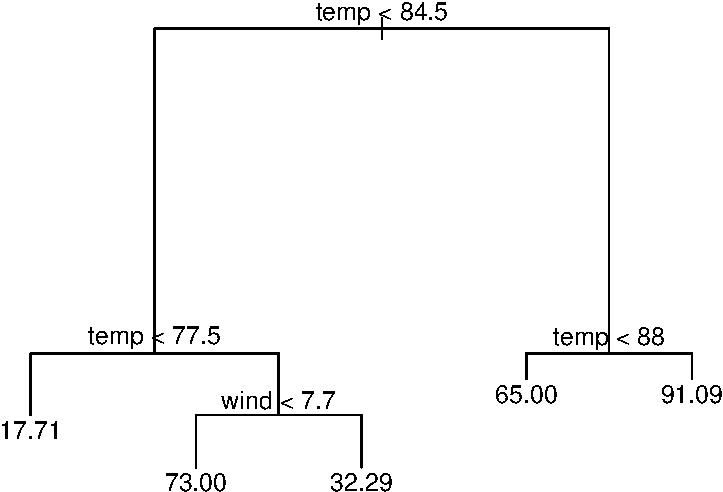
\includegraphics{Rplots_files/figure-latex/unnamed-chunk-7-1.pdf}

\section{Heat map}\label{heat-map}

\begin{Shaded}
\begin{Highlighting}[]
\KeywordTok{library}\NormalTok{(reshape)}
\KeywordTok{head}\NormalTok{(mtcars)}
\NormalTok{carsdf =}\StringTok{ }\KeywordTok{data.frame}\NormalTok{(}\KeywordTok{scale}\NormalTok{(mtcars))}
\NormalTok{carsdf}\OperatorTok{$}\NormalTok{model =}\StringTok{ }\KeywordTok{rownames}\NormalTok{(mtcars)}
\NormalTok{cars_melt =}\StringTok{ }\KeywordTok{melt}\NormalTok{(carsdf, }\DataTypeTok{id.vars =} \StringTok{"model"}\NormalTok{)}

\KeywordTok{ggplot}\NormalTok{(cars_melt, }\KeywordTok{aes}\NormalTok{(}\DataTypeTok{x =}\NormalTok{ variable, }\DataTypeTok{y =}\NormalTok{ model)) }\OperatorTok{+}\StringTok{ }\KeywordTok{geom_raster}\NormalTok{(}\KeywordTok{aes}\NormalTok{(}\DataTypeTok{fill =}\NormalTok{ value)) }\OperatorTok{+}\StringTok{ }
\StringTok{    }\KeywordTok{labs}\NormalTok{(}\DataTypeTok{title =} \StringTok{"Heat Map"}\NormalTok{) }\OperatorTok{+}\StringTok{ }\KeywordTok{scale_fill_continuous}\NormalTok{(}\DataTypeTok{name =} \StringTok{"Value"}\NormalTok{) }\OperatorTok{+}\StringTok{ }\KeywordTok{theme_minimal}\NormalTok{()}
\end{Highlighting}
\end{Shaded}

\includegraphics{Rplots_files/figure-latex/heat-1.pdf}

\begin{verbatim}
##                    mpg cyl disp  hp drat    wt  qsec vs am gear carb
## Mazda RX4         21.0   6  160 110 3.90 2.620 16.46  0  1    4    4
## Mazda RX4 Wag     21.0   6  160 110 3.90 2.875 17.02  0  1    4    4
## Datsun 710        22.8   4  108  93 3.85 2.320 18.61  1  1    4    1
## Hornet 4 Drive    21.4   6  258 110 3.08 3.215 19.44  1  0    3    1
## Hornet Sportabout 18.7   8  360 175 3.15 3.440 17.02  0  0    3    2
## Valiant           18.1   6  225 105 2.76 3.460 20.22  1  0    3    1
\end{verbatim}

\section{Correlogram}\label{correlogram}

The \texttt{ozone} data:

\begin{Shaded}
\begin{Highlighting}[]
\KeywordTok{library}\NormalTok{(faraway)}
\KeywordTok{data}\NormalTok{(ozone)}
\KeywordTok{library}\NormalTok{(corrplot)}
\NormalTok{ozonecorr =}\StringTok{ }\KeywordTok{cor}\NormalTok{(ozone)}
\KeywordTok{corrplot}\NormalTok{(ozonecorr)}
\end{Highlighting}
\end{Shaded}

\includegraphics{Rplots_files/figure-latex/corrplot-1.pdf}

\begin{Shaded}
\begin{Highlighting}[]
\KeywordTok{library}\NormalTok{(corrgram)}
\KeywordTok{corrgram}\NormalTok{(ozone, }\DataTypeTok{upper.panel =}\NormalTok{ panel.conf)}
\end{Highlighting}
\end{Shaded}

\includegraphics{Rplots_files/figure-latex/corrplot-2.pdf}


\end{document}
